En este ejemplo, los datos disponibles presentan un comportamiento estacional,
evidenciado por los picos máximos y mínimos que se repiten periódicamente a lo
largo del tiempo, como se muestra en la \cref{fig:season-data}.
Para predecir la demanda del primer trimestre del año siguiente
(correspondiente a los valores 16, 17, 18, 19 y 20), es necesario
desestacionalizar los datos.
Para ello, se utilizó el método de promedios móviles.

\begin{figure}[htpb!]
  \centering
  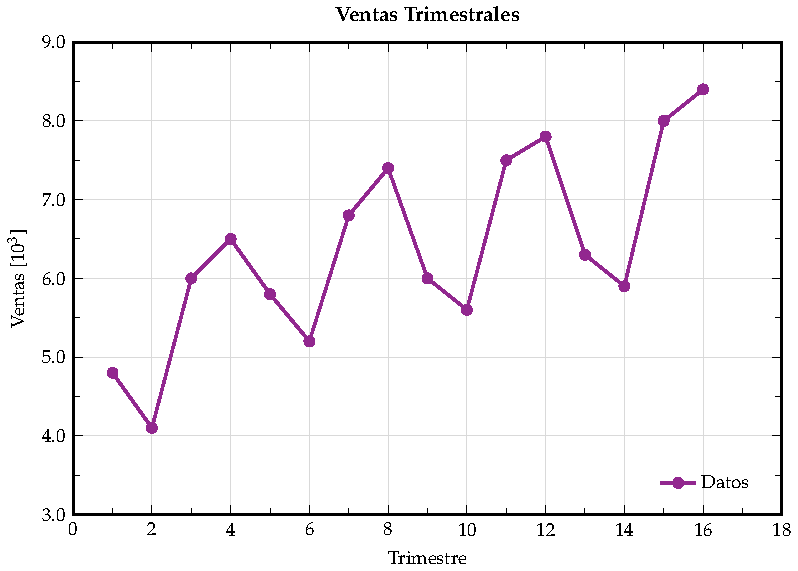
\includegraphics[width=\columnwidth]{../Figures/season-data.pdf}
  \caption{Datos de ventas registrados.}
  \label{fig:season-data}
\end{figure}

Este método consiste en calcular el promedio de cuatro valores consecutivos de
demanda, comenzando con los correspondientes a los trimestres 1, 2, 3 y 4,
luego con los trimestres 2, 3, 4 y 5, y así sucesivamente hasta llegar al
promedio de los trimestres 13, 14, 15 y 16.
Cada uno de estos promedios se ubica en la posición intermedia entre el segundo
y el tercer valor del grupo correspondiente.
Sin embargo, dado que esa ubicación no coincide con ningún trimestre específico,
es necesario calcular un nuevo promedio entre cada par de promedios consecutivos
ya obtenidos.
El resultado de este segundo promedio se asigna a la fila situada entre ambos
valores originales.
Estos nuevos valores corresponden a la columna denominada \textit{Promedio centrado}
en la \cref{tab:table}.

A continuación, se divide cada valor de demanda entre su respectivo promedio
centrado, obteniendo así un coeficiente por cada trimestre de demanda.
Por ejemplo, el coeficiente de 1.1 corresponde al trimestre de demanda 3, mientras
que el valor 0.97 se asocia al trimestre de demanda 1, y no al 5, debido a que
cada trimestre del año agrupa cuatro valores de demanda.
Una vez realizados estos cálculos, se agrupan los coeficientes según el
trimestre al que pertenecen y se calcula el promedio de cada grupo.
De esta manera, se obtienen los coeficientes de desestacionalización, que son
únicamente cuatro.

Para obtener los valores de demanda desestacionalizada, se debe dividir cada
valor de demanda entre su coeficiente de desestacionalización correspondiente
(ya sea del primer, segundo, tercer o cuarto trimestre).
Una vez desestacionalizados, los datos muestran un comportamiento lineal, como
se observa en la \cref{fig:out-season-data}.
Por lo tanto, se procede a realizar un ajuste lineal, del cual se obtiene la
\cref{eq:regression}.

\begin{equation}
  y = 0.148x + 5.101
  \label{eq:regression}
\end{equation}

\begin{figure}[htpb!]
  \centering
  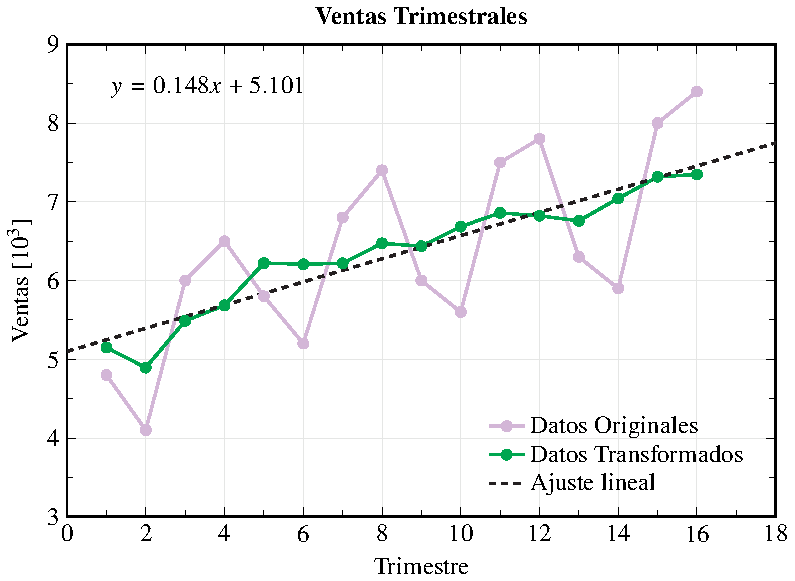
\includegraphics[width=\columnwidth]{../Figures/out-season-data.pdf}
  \caption{Regresión lineal obtenida.}
  \label{fig:out-season-data}
\end{figure}

Con la \cref{eq:regression}, se calculan los valores de demanda
desestacionalizada para los trimestres 17, 18, 19 y 20, sustituyendo en la
ecuación el valor de $x$ por cada uno de estos trimestres.
A los resultados obtenidos se les añade el margen de error, el cual se calcula
mediante la \cref{eq:error-margin}, donde \( y \) corresponde a los valores de
demanda desestacionalizada, \( n \) el numero datos (16), \( a, b \)
el intercepto con el eje vertical y la pendiente de la linea, \(5.101\) y \(0.148 \)
respectivamente.

\begin{equation}\label{eq:error-margin}
  m_r = \sqrt{\frac{\sum y^2 - a(\sum y - b\sum xy)}{n-2}}
\end{equation}

Una vez obtenidos los valores de demanda desestacionalizada para el primer
trimestre del año siguiente, cada uno debe multiplicarse por su coeficiente de
desestacionalización correspondiente.
De este modo, se obtienen los valores de demanda real para dichos trimestres.
En la \cref{fig:prediction} se muestra la gráfica con los valores de demanda
correspondientes a los cinco años presentados en la \cref{tab:table}.

\begin{figure}[htpb!]
  \centering
  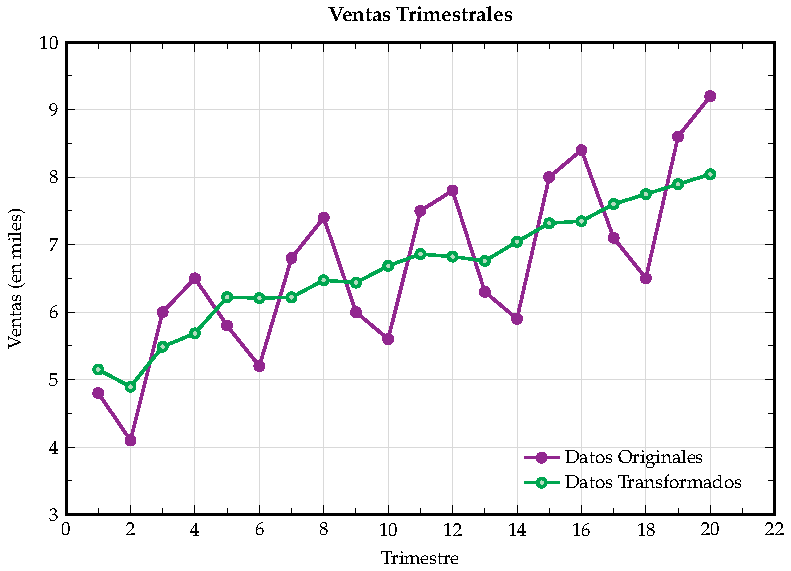
\includegraphics[width=\columnwidth]{../Figures/prediction-data.pdf}
  \caption{Predicción del siguiente año.}
  \label{fig:prediction}
\end{figure}

\begin{table*}[htbp!]
	\centering
	\pgfplotstabletypeset[
	col sep=tab,
	header=false,
	columns/0/.style={
		column name={Año},
		column type=c,
	},
	columns/1/.style={
		column name={Trimestre},
		column type=c,
	},
	columns/2/.style={
		column name={Ventas [\(10^3\)]},
		fixed zerofill,
		precision=1,
	},
	columns/3/.style={
		column name={Promedio Anual},
		fixed zerofill,
		precision=2,
	},
	columns/4/.style={
		column name={Promedio Centrado},
		fixed zerofill,
		precision=3,
	},
	columns/5/.style={
		column name={Valores Irregulares},
		fixed zerofill,
		precision=3,
	},
	columns/6/.style={
		column name={Índice Estacional},
		fixed zerofill,
		precision=2,
	},
	columns/7/.style={
		column name={Ventas Desestacionalizadas},
		fixed zerofill,
		precision=2,
	},
	every head row/.style={
		before row=\toprule, after row=\midrule
	},
	every last row/.style={after row=\bottomrule},
	every even row/.style={
		before row={\rowcolor[gray]{0.95}}
	},
	every nth row={4}{
		before row={\midrule\rowcolor[gray]{0.95}}
	}
	]{./Tables/table.tsv}
	\vspace{2pt}
	\caption{Promedios, índices y predicciones calculadas.}
	\label{tab:table}
\end{table*}


